%
% 54-hgruppe.tex -- Homologiegruppe
%
% (c) 2026 Prof Dr Andreas Müller
%
\subsection{Homologiegruppe}
Im Abschnitt~\ref{buch:integration:homologie:subsection:homologie}
haben wir die Homologierelation durch die Umlaufzahl um Punkte,
die ausserhalb des Definitionsgebietes liegen, definiert.
%
% fig-raender.tex
%
% (c) 2026 Prof Dr Andreas Müller
%
\begin{figure}
\centering
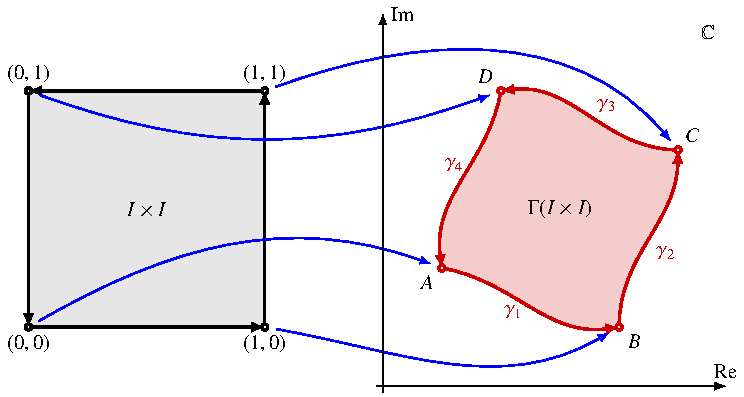
\includegraphics{chapters/030-integration/images/raender.pdf}
\caption{Zweidimensionale Kette und Rand.
\label{buch:integration:homologie:fig:raender}}
\end{figure}
%
Unter Verwendung der Homotopieeigenschaft können wir aber auch eine
algebraische Definition aufbauen.
Dazu konstruieren wir zunächst die zweidimensionalen Ketten.

\begin{definition}[Zweidimensionale Ketten]
Eine \emph{zweidimensionale Kette} ist eine formale Linearkombination
von Abbildungen 
\[
\Gamma
\colon
I\times I \to U
:
(s,t) \mapsto \Gamma(s,t)
\]
Die Menge der zweidimensionalen Ketten wird mit
\[
C_2
=
C_2(U)
=
\biggl\{
\sum_{k=1}^n c_k\Gamma_k
\;
\bigg|
\;
c_k\in\mathbb{Z}, \Gamma_k\colon I\times I\to U
\biggr\}
\]
bezeichnet.
Der \emph{Randoperator} für zweidimensionale Ketten ist die lineare
Abbildung, die einer einzelnen Abbildung $\Gamma$ die Summe
\[
\partial \Gamma
=
\gamma_1
+
\gamma_2
+
\gamma_3
+
\gamma_4
\]
zuordnet, wobei die $\gamma_k$ die Wege
\[
\renewcommand{\arraycolsep}{2pt}
\begin{array}{rlcl}
\gamma_1 &\colon I \to U&:&t\mapsto \Gamma(t,0)\\
\gamma_2 &\colon I \to U&:&t\mapsto \Gamma(1,t)\\
\gamma_3 &\colon I \to U&:&t\mapsto \Gamma(1-t,1)\\
\gamma_4 &\colon I \to U&:&t\mapsto \Gamma(0,1-t)
\end{array}
\]
sind.
\end{definition}

Die Wege $\gamma_k$ sind in
Abbildung~\ref{buch:integration:homologie:fig:raender} dargestellt.
$\gamma_1$ ist der Weg auf dem Rand von $A$ nach $B$,
$\gamma_2$ ist das Randstück von $B$ nach $C$,
$\gamma_3$ das Randstück von $C$ nach $D$ und
$\gamma_4$ das Randstück von $D$ zurück nach $A$.
Es ist offensichtlich, dass die vier Wegstücke einen geschlossenen
Weg bilden und dass daher $\partial\partial \Gamma=0$ ist.
Die Ketten $\gamma_1$ und $-\gamma_2-\gamma_3-\gamma_4$ sind homolog,
da die $\gamma_1+\gamma_2+\gamma_3+\gamma_4$ ein geschlossener
Weg ist.

Eine Abbildung $\Gamma\colon I\times I\to U$ kann man auch als
eine Homotopie zwischen den Wegen $\gamma_1$ und $\gamma
=
\gamma_4^{-1}\cdot\gamma_3^{-1}\cdot\gamma_2^{-1}$ lesen.
Auch die Zusammensetzung der roten und blauen Kurven in 
Abbildung~\ref{buch:integration:homologie:fig:residuum}
lässt sich als Rand einer Abbildung $\Gamma\colon I\times I\to U$
ansehen, die das Einheitsquadrat auf das hellrot ausgefüllte Gebiet
abbildet.
Die Tatsache, dass $\gamma$ und $-\gamma_1$ dort homolog sind, folgt
also daraus, dass sich die Kurven mithilfe einer zweidimensionalen
Kette (mit einer einzigen Abbildung $\Gamma$) ``ausfüllen'' lässt.

\begin{definition}[Ränder]
Die Menge
\[
B_1
=
B_1(U)
=
\biggl\{
\partial c
\;
\bigg|
\;
c = \sum_{k=1}^n c_k \Gamma_k\in C_2(U)
\biggr\}
=
\partial C_2(U)
\]
heisst die Menge der \emph{Ränder}.
\index{Rander@Ränder}%
\end{definition}

Die Beispiele, insbesondere auch die
Abbildung~\ref{buch:integration:homologie:fig:residuum}, zeigen,
dass homologe geschlossene Kurven sich durch den Rand einer
zweidimensionalen Kette unterscheiden.
Die Ränder $B_1$ von zweidimensionalen Ketten definieren also
eine Äquivalenzrelation von Zyklen.
Zwei Zyklen $c_1, c_2\in Z_1$ sind homolog, wenn es eine
zweidimensionale Kette $d\in C_2$ gibt derart, dass $c_1-c_2=\partial d$.
Die Zyklen unterscheiden sich daher um einen Rand.
Die Menge
\[
c+B_1(U)
=
\{
c+\partial d
\mid
d\in C_2(U)
\}
\]
besteht also aus den Zyklen, die zu $c$ homolog sind.
Diese Mengen sind die Äquivalenzklassen von Zyklen unter Äquivalenzrelation
der Homologie von Zyklen.

\begin{definition}[Homologiegruppe]
\label{buch:integration:homologie:definition:homologiegruppe}
Die Menge
\[
H_1(U)
=
Z_1(U)/B_1(U)
=
\{
c + \partial C_2
\mid
c\in Z_1(U)
\}
=
\{
c+ B_1(U)
\mid
c\in Z_1(U)
\}
\]
der Äquivalenzklassen homologer Zyklen heisst die erste
\emph{Homologiegruppe}.
\index{Homologiegruppe}%
\end{definition}

Die Definition~\ref{buch:integration:homologie:definition:homologiegruppe}
spricht von einer Gruppe, es muss also noch verifiziert
werden, dass die Addition von Zyklen ein Gruppenoperation auf $H_1(Z)$ ist.
Die Operationen werden auf den Repräsentanten in einer Äquivalenzklasse
definiert.
Daher muss gezeigt werden, dass es nicht auf die Wahl des Repräsentaten
ankommt, oder genauer, dass die Rechenoperationen mit verschiedene
Repräsentanten zu homologen Resultaten führen.
Sind $c$ und $c+\partial d$ Repräsenten der Menge der zu $c$
homologen Zyklen, dann sind ihre additiven Inversen
\(
-c
\)
und
\(
-c-\partial d
\).
Der Unterschied ist
\[
-c
-(
-c-\partial d
)
=
\partial d \in B_1.
\]
Die beiden Repräsentaten von $-c$ sind also homolog und repräsentieren
die selbe Äquivalenzklasse.
Für die Addition betrachten wir Repräsentanten $a$ und $a+\partial d_a$
bzw.~$b$ und $b+\partial d_b$.
Die Summen unterscheiden sich um
\[
(a+b)-(a+\partial d_a+b+\partial d_b)
=
-\partial(d_a+d_b)
\in
B_1(U),
\]
wobei die letzte Umformung aus der Linearität des Randoperators folgt.
Die beiden Repräsentanten der Summe $a+b$ sind daher homolog.

Ränder sind zusammenziehbare Kurven, das Wegintegral über einen
Rand verschwindet daher immer.
Dies zeigt erneut, dass Wegintegrale über homologe Zyklen gleich sind.
Das Wegintegral einer Funktion $f$ definiert also eine lineare Abbildung
von Klassen homologer Zyklen.

\begin{satz}
Die Abbildung
\[
\oint f(z)\,dz
\colon
H_1(U) \to \mathbb{C}
:
c
\mapsto
\oint_c f(z)\,dz
\]
ist eine lineare Abbildung.
\end{satz}
